\section{動作與控制}
\label{sec:motion}

\subsection{從輸入到動作}

程式的主迴圈是一個固定約 60 Hz 的 \lstinline|glutTimerFunc|。
會定期推進世界的時間，並且處理玩家的輸入、更新機器人的狀態、模擬世界的物理、以及繪製畫面。

每個 tick 中，玩家的按鍵先被轉成一個 \lstinline|Intent|，描述「想做什麼」：
前後左右的移動量、是否跑步、是否跳躍、想切換的姿勢，以及視線方向。
機器人收到 \lstinline|Intent| 後依序處理：

\begin{enumerate}
    \item 身體朝向設為視線的 yaw，轉彎因此由視角控制
    \item 處理姿勢切換的請求，並推進轉換的進度
    \item 依目前的姿勢決定目標速度，交給物理模擬器計算位移與碰撞（第~\ref{sec:collision} 節）
    \item 以實際移動的距離推進走路的步伐
\end{enumerate}

繪製時再依姿勢與步伐算出各關節的角度。
這樣的分工讓「想做什麼」與「能做到什麼」分開：鍵盤只產生意圖，速度上限、姿勢限制與碰撞都由機器人本身決定。

\subsection{姿勢切換}

機器人有站立、潛行、坐下三種姿勢（圖~\ref{fig:stances}），每種姿勢是一組關節角度加上 rootOffset：
\begin{itemize}
    \item \textbf{站立}：所有關節為 $0^\circ$，髖部高度等於腿長 $L = 13$ px。
    \item \textbf{潛行}：大腿往前抬 $60^\circ$、膝蓋彎 $60^\circ$，軀幹前傾 $30^\circ$、脖子回抬 $30^\circ$ 讓視線維持水平；髖部降到 $\frac{\sqrt{3}}{2} L$。
    \item \textbf{坐下}：大腿往前抬 $90^\circ$ 並向外張開 $15^\circ$，髖部降到大腿厚度的一半，正好坐在地上。
\end{itemize}

姿勢的轉換記錄為起點 \lstinline|from|、終點 \lstinline|to| 與進度 $t \in [0, 1]$，固定花 0.5 秒完成；
轉換中每個關節角度與 rootOffset 都以 $t$ 在兩個姿勢間線性內插。
轉換途中只接受「折返」：若要求回到起點，就交換 \lstinline|from| 與 \lstinline|to| 並把進度改為 $1 - t$，
動作會從目前的位置原路退回而不會跳動；要求第三種姿勢則忽略，直到這次轉換結束。
轉換中機器人不能移動，碰撞箱的大小也隨 $t$ 內插（第~\ref{sec:collision} 節）。

\begin{figure}[htbp]
    \centering
    \begin{subfigure}[t]{.32\textwidth}
        \centering
        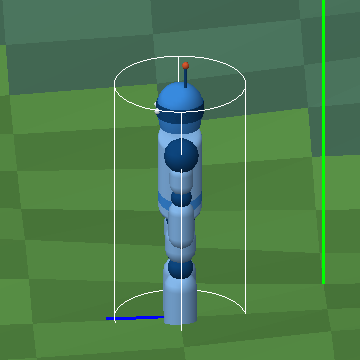
\includegraphics[width=\linewidth]{docs/figures/stance-standing.png}
        \caption{站立}
    \end{subfigure}\hfill
    \begin{subfigure}[t]{.32\textwidth}
        \centering
        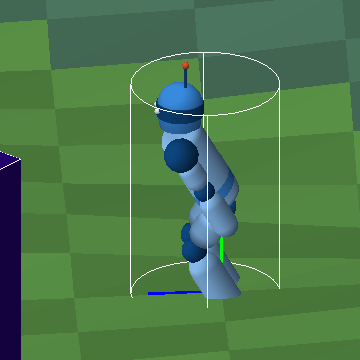
\includegraphics[width=\linewidth]{docs/figures/stance-sneaking.png}
        \caption{潛行}
    \end{subfigure}\hfill
    \begin{subfigure}[t]{.32\textwidth}
        \centering
        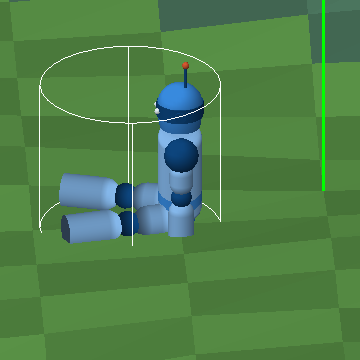
\includegraphics[width=\linewidth]{docs/figures/stance-sitting.png}
        \caption{坐下}
    \end{subfigure}
    \caption{三種姿勢；線框為碰撞箱}
    \label{fig:stances}
\end{figure}

\subsection{走路與跑步}

手腳擺動是參考 Minecraft 動畫，依照水平移動距離長度計算相位。
機器人著地時累積水平移動距離 $d$，並以此計算相位
$$
    \phi = 2\pi \frac{d}{C}, \qquad C = 2 \cdot 2L \sin 25^\circ \approx 1.37 \text{ m},
$$
其中 $C$ 是左右各跨一步走過的距離：大腿前後各擺 $25^\circ$ 時，兩腳張開的前後距離為 $2L \sin 25^\circ$。
另外定義兩個係數：$a$ 是擺動幅度，目標值為「目前速度 / 走路速度」，上限 1.2，停下時為 0；$r \in [0, 1]$ 是跑步的程度，速度超過走路速度時開始增加，達到兩倍時為 1。
各關節在站立姿勢上疊加的 pitch 角度為
\begin{align*}
    \text{髖} & = \pm 25^\circ \sin\phi \cdot a,               & \text{膝} & = -40^\circ \max(0, \pm\cos\phi) \cdot a, \\
    \text{肩} & = \mp 20^\circ \sin\phi \cdot a + 180^\circ r, & \text{肘} & = 15^\circ \cdot a \, (1 - r),
\end{align*}
其中 $\pm$、$\mp$ 的上方符號用於左側、下方用於右側，pitch 正值為往前抬，因此兩腳交替、手與同側的腳反向擺動。
$\cos\phi$ 是 $\sin\phi$ 的變化方向，膝蓋只在大腿正往前擺的那隻腳彎曲，讓腳尖離地。
支撐腳是直的，髖角度為 $\theta = 25^\circ \sin\phi \cdot a$ 時髖部降低 $L(1 - \cos\theta)$，扣在 rootOffset 上，身體就隨步伐起伏。

跑步時雙臂伸直高舉過頭，並向外張開 $20^\circ r$ 成 V 字。
$a$ 與 $r$ 都不直接跳到目標值，而是每個 tick 以 $x \leftarrow x + (x^\ast - x)(1 - e^{-k\,\Delta t})$ 逼近，停下或起跑時手腳會平順地收回或展開；這個式子連續套用兩次 $\Delta t$ 與套用一次 $2\Delta t$ 的結果相同，因此與 tick 頻率無關。

\subsection{轉向與視線}

視線由 yaw 與 pitch 組成。拖曳滑鼠或按 Q、E 改變視線，機器人的身體朝向直接跟著視線的 yaw，這就是轉彎；前進與平移的方向也以視線為準。
視線的 pitch 則交給頭部的 pitch 關節，機器人抬頭、低頭看向相機注視的方向，超過頭部的角度範圍時由關節限制截斷。
自由相機模式下視線不再更新，機器人維持原本的朝向，方便從其他角度觀察。

\subsection{跳躍與重力}

以數值積分模擬重力，每個 tick 先更新速度再更新位移：
\begin{equation*}
    \mathbf{v} \leftarrow \mathbf{v} + \mathbf{a}\,\Delta t, \qquad \mathbf{x} \leftarrow \mathbf{x} + \mathbf{v}\,\Delta t, \qquad \mathbf{a} = (0, -g, 0),\; g = 9.80665 \text{ m/s}^2 .
\end{equation*}
著地時假設摩擦力足夠大，水平速度直接等於目標速度；在空中則只受重力影響，維持起跳時的水平速度，因此在空中無法改變移動方向或加速。
跳躍高度 $h = 0.5$ m，由 $v^2 = 2gh$ 得到起跳的鉛直速度 $v_y = \sqrt{2gh}$。

\subsection{動作限制}

\begin{itemize}[nosep]
    \item \textbf{速度}：站立時走路 1.2 m/s、跑步 3 m/s，潛行 0.6 m/s，坐下或轉換姿勢時為 0；前後與左右同時按下時，合成方向的長度會被限制在 1，斜走不會比直走快。
    \item \textbf{關節角度}：每次計算骨架矩陣前，所有角度都會被截斷到表~\ref{tab:dof} 的範圍；擺動幅度的上限 1.2 也是依髖關節往後的極限 $-30^\circ$ 決定的。
    \item \textbf{姿勢}：只有站立能跑，坐下不能移動或跳躍。
\end{itemize}

\subsection{抓東西}

% TODO: 功能完成後補上
（尚未實作。）
